\documentclass{article}

% Packages for formatting
\usepackage{tcolorbox}
\usepackage{xcolor}
\usepackage{hyperref}
\usepackage{amsmath}
\usepackage{geometry}
\usepackage{tocloft}
\usepackage{colortbl}
\usepackage{graphicx}
\usepackage{lipsum} % For dummy text
\usepackage{listings}

% Change hyperref settings to remove boxes
\hypersetup{
    colorlinks=true,
    linkcolor=black,
    filecolor=black,
    urlcolor=black,
    citecolor=black,
}

% Page layout
\geometry{a4paper, margin=1in}

% Colors
\definecolor{codehighlight}{rgb}{0.36, 0.54, 0.66}
\definecolor{coderule}{rgb}{0.7, 0.7, 0.7}           % Grey frame codebox
\definecolor{codebg}{rgb}{1.0, 1.0, 1.0}             % Background codebox
\definecolor{tableheader}{RGB}{128, 128, 128}        % Grey table header
\definecolor{tablecell}{RGB}{250, 250, 250}          % Table cell
\definecolor{title}{rgb}{0.36, 0.54, 0.66}           % Custom title color


% Code box style
\tcbset{
    colframe=tableheader, % Frame color
    colback=tablecell,    % Background color
    arc=0pt,           % Corner radius
    boxrule=1pt        % Frame thickness
}

% Table of contents
% \renewcommand{\cftbot}{}

% Main document
\begin{document}

% Cover pages
% Cover page
\begin{titlepage}
    \centering
    \vspace{\fill}  % push everything to top

    \thispagestyle{empty} % Remove page numbering

    % Background image
    \newgeometry{left=0cm, right=0cm, top=0cm, bottom=0cm} % Temporarily set margins to 0
    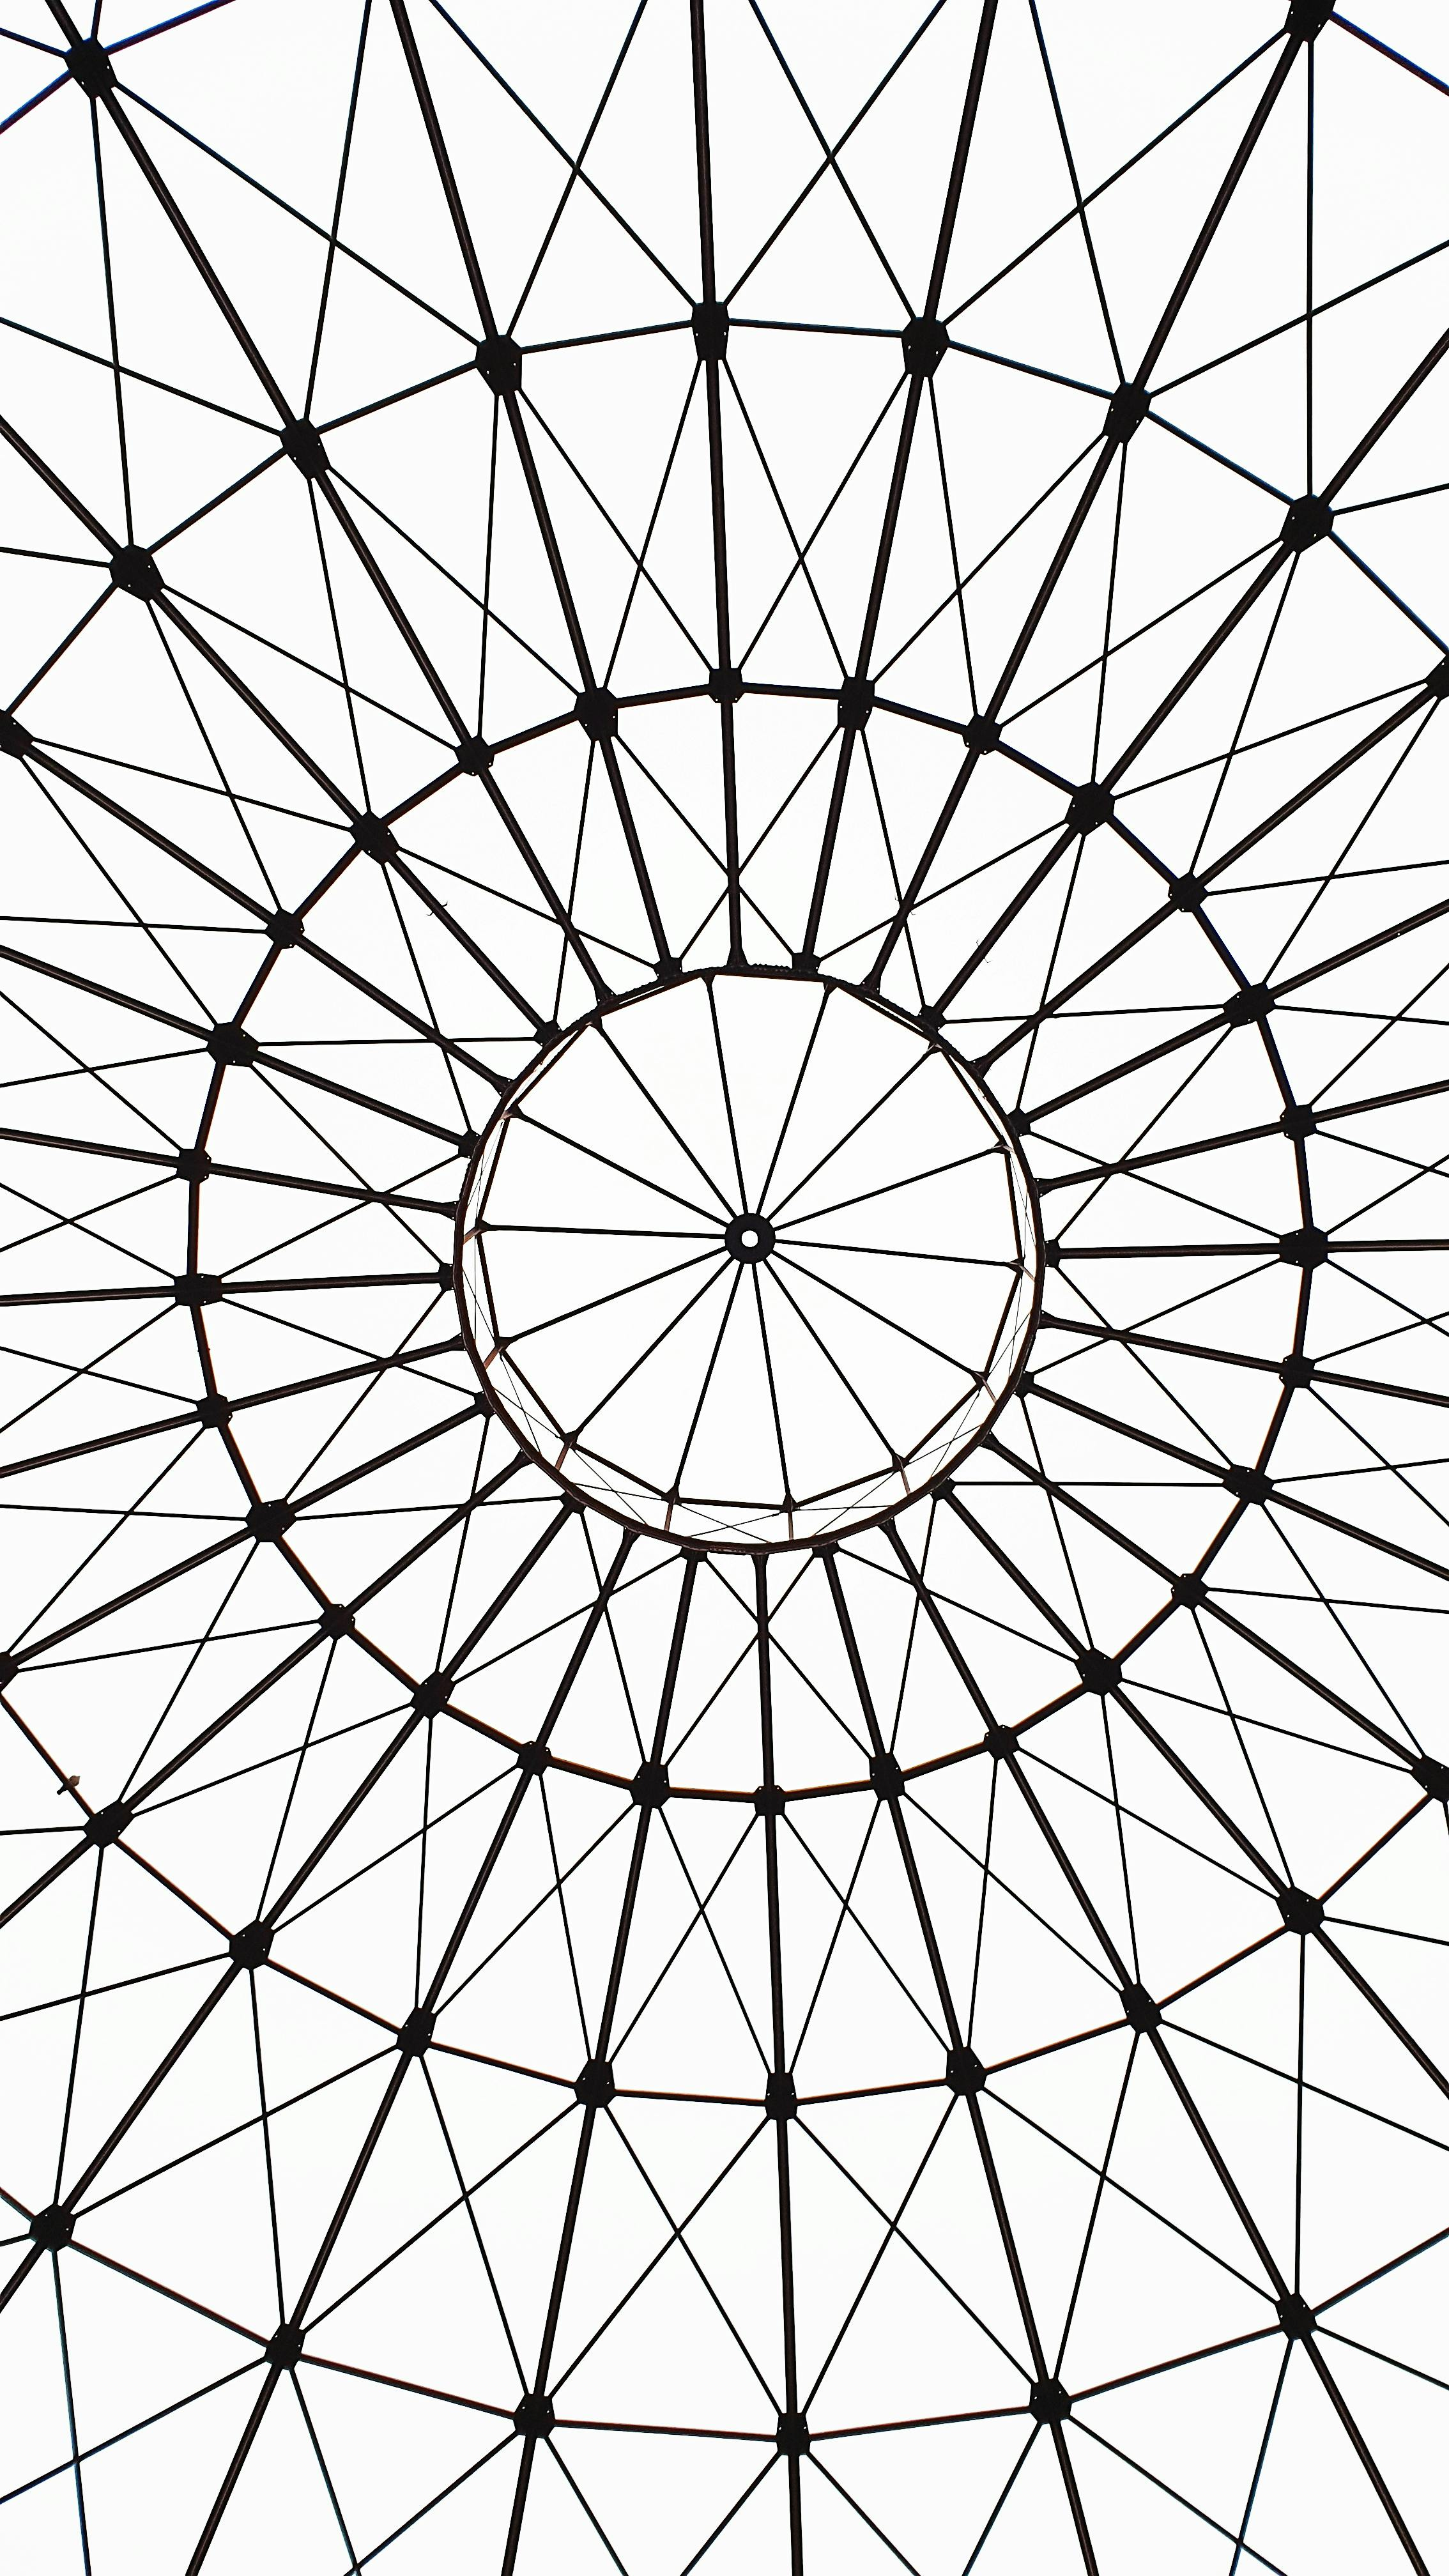
\includegraphics[width=\paperwidth,height=\paperheight]{images/cover.jpg}
    \restoregeometry % Restore the margins

    \vspace{\fill}   % push everything to bottom
\end{titlepage}
% Title page
\begin{titlepage}
    \thispagestyle{empty} % Remove page numbering
    \centering
    \vfill                % push everything to top
    \begin{center}
        {\Huge \textbf{C++ QuestionBank}}\\
        \vspace{1cm}
        {\Large Anchit Mulye}\\
        \vspace{0.5cm}
        {\Large \today}
    \end{center}
    \vfill                % push everything to bottom
\end{titlepage}
\pagenumbering{roman}
% Table of contents
\newpage
\thispagestyle{empty} % Remove page numbering
\title{C++ Question Bank}
\author{Anchit Mulye}
\date{\today}
\maketitle

\tableofcontents
\newpage

% Chapters
\pagenumbering{arabic}
% \section{Introduction}

% Lorem Ipsum is simply dummy text of the printing and typesetting industry. Lorem Ipsum has been the industry's standard dummy text ever since the 1500s, when an unknown printer took a galley of type and scrambled it to make a type specimen book. It has survived not only five centuries, but also the leap into electronic typesetting, remaining essentially unchanged. It was popularised in the 1960s with the release of Letraset sheets containing Lorem Ipsum passages, and more recently with desktop publishing software like Aldus PageMaker including versions of Lorem Ipsum.

\lipsum[1] % Dummy text for illustration

\subsection{Main Section}
\lipsum[2] % Dummy text for illustration

\subsubsection{Subsection}
\lipsum[3] % Dummy text for illustration

\paragraph{Paragraph Heading}
This is a paragraph with a heading. It provides a way to further organize content within a subsection or subsubsection.

\lipsum[4] % Dummy text for illustration

\subsection{Another Main Section}
\lipsum[5] % Dummy text for illustration

\paragraph{Another Paragraph Heading}
This is another paragraph with a heading. You can use multiple paragraph headings within a subsection or subsubsection to structure your content.

\lipsum[6] % Dummy text for illustration

\lipsum[7] % Dummy text for illustration

\lipsum[8] % Dummy text for illustration

\lipsum[9] % Dummy text for illustration
% \chapter*{Part I. Language}

\section{Language Basics}

\subsection{Characteristics of C}
C is a general-purpose, procedural language developed by Dennis Ritchie in the 1970s at AT\&T Bell Labs, designed for Unix system development. Key features include:
\begin{itemize}
    \item \textbf{Source Code Portability}: Independent of specific hardware platforms.
    \item \textbf{Close to the Machine}: Efficient low-level operations.
    \item \textbf{Efficiency}: Optimized for performance.
\end{itemize}
C’s design, influenced by BCPL and B, includes various data types. Its first description by Kernighan and Ritchie (K\&R) became the standard reference. C’s portability is enhanced by a core language with minimal hardware dependencies and a comprehensive standard library for functions like I/O and memory management.\\
C is widely used in system programming and embedded systems, as well as high-level applications like word processors and databases.\\


\subsection{The Structure of C Programs}
C programs are composed of functions, with \texttt{main()} as the entry point. Functions execute sequentially and can call others. Programs can use the standard library or custom functions, with portability considerations for nonstandard libraries.
\begin{tcolorbox}[title=Example structure of C program]
\begin{verbatim}
#include <stdio.h>              // Preprocessor directive
double circularArea(double r);  // Function prototype

int main() {                    // Main function
    double radius = 1.0, area = 0.0;
    printf("Areas of Circles\n\n");
    area = circularArea(radius);
    printf("%10.1f     %10.2f\n", radius, area);
    radius = 5.0;
    area = circularArea(radius);
    printf("%10.1f     %10.2f\n", radius, area);
    return 0;
}
\end{verbatim}
\end{tcolorbox}


\subsection{Source Files}
C programs consist of function definitions, global declarations, and preprocessing directives. Small programs use a single source file, while larger ones are split into multiple files, typically structured as follows:
\begin{itemize}
    \item \textbf{Preprocessor Directives}
    \item \textbf{Global Declarations}
    \item \textbf{Function Definitions}
\end{itemize}
Source files, labeled with the \texttt{.c} suffix, are modular and can be compiled separately. Functions are logically grouped, such as user interface functions.


\subsection{Comments}
Use comments generously in C programs for documentation. There are two types:
\begin{itemize}
    \item \textbf{Block Comments}: \texttt{/* ... */} for multi-line comments.\\
    within a line:
    \begin{tcolorbox}[]
    \begin{verbatim}
    int open(const char *name, int mode, ... /* int permissions */);
    \end{verbatim}
    \end{tcolorbox}
    \item \textbf{Line Comments}: \texttt{//} for single-line comments (added in C99, also known as "C++-style").\\
    in two-column format:
    \begin{tcolorbox}[]
    \begin{verbatim}
    const double pi = 3.1415926536; // Pi is constant
    \end{verbatim}
    \end{tcolorbox}
\end{itemize}

\begin{tcolorbox}[arc=5pt, boxrule=2pt, title=Notes]
    Inside strings or character constants, /* and // do not start comments:
    \begin{verbatim}
    printf("Comments in C begin with /* or //.\n");
    \end{verbatim}   
    \textbf{Nesting Block Comments}: Not allowed. Use block comments to temporarily remove code containing line comments:
    \begin{verbatim}
    /* Temporarily removing two lines:
    const double pi = 3.1415926536; // Pi is constant
    area = pi * r * r               // Calculate the area
    Temporarily removed up to here */
    \end{verbatim}   
    \textbf{Conditional Preprocessor Directive}: To remove sections containing block comments:
    \begin{verbatim}
    #if 0
    const double pi = 3.1415926536; /* Pi is constant */
    area = pi * r * r;              /* Calculate the area */
    #endif
    \end{verbatim}   
\end{tcolorbox}


\subsection{Character Sets}
C distinguishes between the \textbf{translation environment} (where source files are compiled) and the \textbf{execution environment} (where the compiled program runs). Each environment has its own character set:
\begin{itemize}
    \item \textbf{Source Character Set}: Used in C source code.
    \item \textbf{Execution Character Set}: Interpreted by the running program.
\end{itemize}
\textbf{\textit{Basic and Extended Character Sets}} \\
Both the source and execution character sets include:
\begin{itemize}
    \item \textbf{Latin Alphabet}: A-Z, a-z
    \item \textbf{Decimal Digits}: 0-9
    \item \textbf{Punctuation Marks}:
    \begin{lstlisting}[basicstyle=\ttfamily]
    ! " # % & ' ( ) * + , - . / : ; < = > ? [ ] \ ^ _ { | } ~
    \end{lstlisting}
    \item \textbf{Whitespace Characters}: Space, horizontal tab, vertical tab, new line, form feed
\end{itemize}

The \textbf{basic execution character set} also includes:
\begin{itemize}
    \item \textbf{Nonprintable Characters}: null (\texttt{\textbackslash 0}), alert (\texttt{\textbackslash a}), backspace (\texttt{\textbackslash b}), carriage return (\texttt{\textbackslash r})
\end{itemize}
Character codes may vary across implementations, with conditions:

\begin{itemize}
    \item Basic characters must be representable in one byte.
    \item The null character's byte has all bits set to 0.
    \item Digits increment by one sequentially.
\end{itemize}
\textbf{\textit{Wide Characters and Multibyte Characters}} \\
To accommodate diverse languages, C supports:

\begin{itemize}
    \item \textbf{Wide Characters} (\texttt{wchar\_t}): Fixed bit width for each character, suitable for large character sets.
    \item \textbf{Multibyte Characters}: Variable length, used for complex scripts (e.g., UTF-8).
\end{itemize}

C provides functions like \texttt{wctomb()} for conversions between wide and multibyte characters. Example:
\begin{tcolorbox}
\begin{verbatim}
wchar_t wc = L'\x3B1'; // Greek letter alpha 
char mbStr[10] = "";
int nBytes = wctomb(mbStr, wc); // Converts to multibyte
\end{verbatim}
\end{tcolorbox}

\textbf{\textit{Digraphs and Trigraphs}} \\
C provides \textbf{digraphs} and \textbf{trigraphs} as alternative representations for certain punctuation marks, useful when specific characters are not available on all keyboards.
\textbf{\textit{Digraphs}} \\
Digraphs are two-character sequences that represent single characters. They are not interpreted within character constants or string literals.
\begin{table}[h]
\centering
\begin{tabular}{|>{}c|c|}
\hline
\rowcolor{tableheader}
\textbf{Digraph}        & \textbf{Equivale} \\
\hline \texttt{<:}      & \texttt{[} \\
\hline \texttt{:>}      & \texttt{]} \\
\hline \texttt{<\%}     & \texttt{\{} \\
\hline \texttt{\%>}     & \texttt{\}} \\
\hline \texttt{\%:}     & \texttt{\#} \\
\hline \texttt{\%:\%:}  & \texttt{\#\#} \\
\hline
\end{tabular}
\caption{Digraphs}
\end{table}
\begin{tcolorbox}[title=Example with digraphs]
\begin{verbatim}
int arr<::> = <% 10, 20, 30 %>;
printf("The second array element is <%d>.\n", arr<:1:>);
\end{verbatim}
\end{tcolorbox}
\textbf{\textit{Trigraphs}} \\
Trigraphs are three-character sequences starting with two question marks and represent single characters.
\begin{table}[h]
\centering
\begin{tabular}{|>{}c|c|}
\hline
\rowcolor{tableheader}
\textbf{Trigraph}       & \textbf{Equivale} \\
\hline \texttt{??(}     & \texttt{[} \\
\hline \texttt{??)}     & \texttt{]} \\
\hline \texttt{??<}     & \texttt{\{} \\
\hline \texttt{??>}     & \texttt{\}} \\
\hline \texttt{??=}     & \texttt{\#} \\
\hline \texttt{??/}     & \texttt{\textbackslash} \\
\hline \texttt{??!}     & \texttt{|} \\
\hline \texttt{??'}     & \texttt{\textasciicircum} \\
\hline \texttt{??-}     & \texttt{\textasciitilde} \\
\hline
\end{tabular}
\caption{Trigraphs}
\end{table}
Trigraphs are translated in the first phase of compilation and can appear anywhere, including character constants, string literals, and comments.
\begin{tcolorbox}[title=Example with trigraphs]
\begin{verbatim}
printf("Cancel| `???(y/n)` ");
\end{verbatim}
\end{tcolorbox}
To prevent a trigraph interpretation, escape the question marks:
\begin{tcolorbox}
\begin{verbatim}
printf("Cancel\?\?\?(y/n) ");
\end{verbatim}
\end{tcolorbox}
Additional Punctuation Substitutes
The header file iso646.h defines macros for logical and bitwise operators, e.g., and for \&\& and xor for \textasciicircum.

\subsection{Identifiers}



\subsection{How the C Compiler Works}
The compiling process involves eight logical steps, which can be combined by a compiler:
\begin{enumerate}
    \item \textbf{Character Conversion}: Characters from the source file are converted into the source character set. End-of-line indicators are replaced, and trigraph sequences are converted to single characters.
    \item \textbf{Line Continuation}: Backslashes followed by a newline are deleted, allowing directives to continue on the next line.
    \item \textbf{Tokenization}: The source file is broken into preprocessor tokens and whitespace. Comments are treated as a single space.
    \item \textbf{Preprocessing}: Preprocessor directives are executed, and macro calls are expanded. This step applies to included files as well.
    \item \textbf{Character Set Conversion}: Characters in constants and literals are converted to the execution character set.
    \item \textbf{String Concatenation}: Adjacent string literals are concatenated into a single string.
    \item \textbf{Compilation}: The compiler analyzes the tokens and generates machine code.
    \item \textbf{Linking}: The linker resolves references to external objects/functions and generates the executable file. Unresolved references are taken from libraries.
\end{enumerate}



Some mathematical equations:

\begin{equation}
    E = mc^2
\end{equation}

\begin{equation}
    \frac{d}{dx} \left( e^{x} \right) = e^{x}
\end{equation}

\begin{equation}
    \int_{a}^{b} x^2 \, dx = \left[ \frac{x^3}{3} \right]_{a}^{b}
\end{equation}

\begin{equation}
    \vec{F} = m \vec{a}
\end{equation}

\begin{equation}
    \sigma = \frac{F}{A}
\end{equation}

\begin{equation}
    \sum_{n=1}^{N} n = \frac{N(N+1)}{2}
\end{equation}
\section{Types}

\subsection{Typology}
\subsection{Integer Types}
\subsection{Floating-Point Types}
\subsection{Complex Floating-Point Types (C99)}
\subsection{Enumerated Types}
\subsection{The Type Void}


This is a coding section using tcolorbox for code examples.

\subsection{Python Code}
\begin{tcolorbox}[title=Python Code Example]
\begin{verbatim}
def hello_world():
    print("Hello, World!")
\end{verbatim}
\end{tcolorbox}

\subsection{C++ Code}
\begin{tcolorbox}[title=C++ Code Example]
\begin{verbatim}
#include <iostream>

int main()
{
    std::cout << "Hello, World!" << std::endl;
}
\end{verbatim}
\end{tcolorbox}

\subsection{JavaScript Code}
\begin{tcolorbox}[title=JavaScript Code Example]
\begin{verbatim}
function helloWorld() {
    console.log("Hello, World!");
}
\end{verbatim}
\end{tcolorbox}
\section{Literals}

\subsection{Integer Constants}
\subsection{Floating-Point Constants}
\subsection{Character Constants}
\subsection{String Literals}

This section contains various text formatting settings in Latex.

\subsection{Font Styles}

\textbf{This is bold text.}\\
\textit{This is italic text.}\\
\underline{This is underlined text.}\\
\texttt{This is typewriter (monospaced) text.}\\
\textsc{This is small caps text.}\\
\emph{This is emphasized text.}

\subsection{Font Sizes}

\tiny{This is tiny text.}\\
\scriptsize{This is scriptsize text.}\\
\footnotesize{This is footnotesize text.}\\
\small{This is small text.}\\
\normalsize{This is normal size text.}\\
\large{This is large text.}\\
\Large{This is larger text.}\\
\LARGE{This is even larger text.}\\
\huge{This is huge text.}\\
\Huge{This is hugest text.}

\subsection{Text Colors}

\textcolor{red}{This is red text.}\\
\textcolor{blue}{This is blue text.}\\
\textcolor{green}{This is green text.}\\
\textcolor{codehighlight}{This is custom color text.}

\subsection{Combined Formatting}

\textbf{\textit{This is bold and italic text.}}\\
\underline{\textbf{\textit{This is bold, italic, and underlined text.}}}\\
\textcolor{blue}{\textbf{This is bold blue text.}}
\section{Type Conversions}

\subsection{Conversion of Arithmetic Types}
\subsection{Conversion of Nonarithmetic Types}

% Normal Table
\subsection{Simple Table}
\begin{table}[h]
\centering
\begin{tabular}{|>{}c|c|c|}
\hline
\rowcolor{tableheader}
\textbf{Column 1} & \textbf{Column 2} & \textbf{Column 3} \\
\hline Item 1 & Item 2 & Item 3 \\
\hline Item 4 & Item 5 & Item 6 \\
\hline
\end{tabular}
\caption{A simple table}
\end{table}

\subsection{Colored Table}
\begin{table}[h]
\centering
\begin{tabular}{|>{\columncolor{tableheader}}c|c|c|}
\hline
\rowcolor{tableheader}
\textbf{Column 1} & \textbf{Column 2} & \textbf{Column 3} \\
\hline Item 1 & Item 2 & \cellcolor{codehighlight} Item 3 \\
\hline Item 4 & \cellcolor{codehighlight} Item 5 & Item 6 \\
\hline
\end{tabular}
\caption{A colored table}
\end{table}

% Headerless table
\subsection{Headless Table}
\begin{center} % This is same as /centering
\normalsize % or \footnotesize, \scriptsize, \tiny
\begin{tabular}{|c|c|c|}
\hline Item 1 & Item 2 & Item 3 \\
\hline Item 4 & Item 5 & Item 6 \\
\hline Item 7 & Item 8 & Item 9 \\
\hline
\end{tabular}
\end{center}

% Borderless table
\subsection{Borderless Table}
\begin{center} % This is same as /centering
\normalsize % or \footnotesize, \scriptsize, \tiny
\begin{tabular}{ccc}
\hline Item 1 & Item 2 & Item 3 \\
\hline Item 4 & Item 5 & Item 6 \\
\hline Item 7 & Item 8 & Item 9 \\
\hline
\end{tabular}
\end{center}

% Complete Borderless table
\subsection{Complete Borderless Table}
\begin{center} % This is same as /centering
\normalsize % or \footnotesize, \scriptsize, \tiny
\begin{tabular}{ccc}
Item 1 & Item 2 & Item 3 \\
Item 4 & Item 5 & Item 6 \\
Item 7 & Item 8 & Item 9 \\
\end{tabular}
\end{center}

% Normal Table color
\subsection{Headless Table with Alternating Row Colors}
\raggedright
\large
\begin{tabular}{|c|c|c|}
\hline
\rowcolor{codehighlight} Item 1 & Item 2 & Item 3 \\
\hline Item 4 & Item 5 & Item 6 \\
\hline
\rowcolor{codehighlight} Item 7 & Item 8 & Item 9 \\
\hline
\end{tabular}

\section{Expressions and Operators}

\subsection{How Expessions Are Evaluated}
\subsection{Operators in Detail}
\subsection{Constant Expessions}
\section{Statements}

\subsection{Expression Statements}
\subsection{Block Statements}
\subsection{Loops}
\subsection{Selection Statements}
\subsection{Unconditional Jumps}
\section{Functions}

\subsection{Function Definitions}
\subsection{Function Declarations}
\subsection{How Functions Are Executed}
\subsection{Pointers as Arguments and Return Values}
\subsection{Inline Functions}
\subsection{Variable Numbers of Arguments}
\section{Arrays}

\subsection{Defining Arrays}
\subsection{Accessing Array Elements}
\subsection{Initializing Arrays}
\subsection{Strings}
\subsection{Mulidimensional Arrays}
\subsection{Arrays as Arguments of Functions}
\section{Pointers}

\subsection{Declaring Pointers}
\subsection{Operations with Pointers}
\subsection{Pointers and Type Qualifiers}
\subsection{Pointers to Arrays and Arrays of Pointers}
\subsection{Pointers to Functions}

\section{Structure, Unions and Bit-Fields}

\subsection{Structures}
\subsection{Unions}
\subsection{Bit-Fields}

\section{Declarations}

\subsection{General Syntax}
\subsection{Type Names}
\subsection{typedef Declarations}
\subsection{Linkage of Identifiers}
\subsection{Storage Duration of Objects}
\subsection{Initiazation}
\section{Dynamic Memory Management}

\subsection{Allocating Memory Dynamically}
\subsection{Characteristics of Allocated Memory}
\subsection{Resizing and Releasing Memory}
\subsection{An All-Purpose Binary Tree}
\section{Input and Output}

\subsection{Streams}
\subsection{Files}
\subsection{Opening and Closing Files}
\subsection{Reading and Writing}
\subsection{Random File Access}
\section{Preprocessing Directives}

\subsection{Inserting the Contents of Header Files}
\subsection{Defining and Using Macros}
\subsection{Conditional Compiling}
\subsection{Defining Line Numbers}
\subsection{Generating Error Messages}
\subsection{The \#pragma Directive}
\subsection{The \_Pragma Operator}
\subsection{Predefined Macros}
% \include{chapters/chapter15}
% \include{chapters/chapter16}
% References Section
\section{References}

\begin{enumerate}

% Book example
\item Smith, J. D. (2009). \textit{The Art of Writing}. Random House.
% Edited book example
\item Smith, A. B. (Ed.). (2010). \textit{Advances in Linguistics}. Cambridge University Press.
% Journal article example (print)
\item Jones, S. C., \& Davis, R. J. (2017). Understanding cultural intelligence. \textit{Journal of Cross-Cultural Psychology, 48}(4), 493-514. \url{https://doi.org/10.1177/0022022117704302}
% Journal article example (online)
\item Roberts, T. F., \& Hidajat, M. (2020). Exploring the impact of social media on adolescent development. \textit{Journal of Adolescent Research, 35}(2), 187-210. \url{https://doi.org/10.1177/0743558420913356}
% Website example with author
\item Davis, M. (2018). Understanding climate change. Retrieved from \url{https://www.example.com/climate-change}
% Website example without author
\item National Institute of Mental Health. (2021). Depression in children and teens. Retrieved from \url{https://www.nimh.nih.gov/health/topics/depression}
% Chapter in edited book example
\item Green, R. T. (2012). Language development in early childhood. In P. H. Smith (Ed.), \textit{Language Acquisition: Theoretical Approaches} (pp. 45-68). Oxford University Press.
% Newspaper article example
\item Smith, J. (2022, June 15). New trends in technology. \textit{The New York Times}, pp. A1, A10.
% Report or government document example
\item United Nations. (2015). \textit{Sustainable Development Goals: 17 Goals to Transform Our World}. Author.
% Conference paper example
\item Brown, L. M. (2019). Education reform in the digital age. Paper presented at the Annual Conference of the American Educational Research Association, Toronto, Canada.
% Thesis or dissertation example
\item Johnson, S. L. (2018). \textit{Understanding leadership in nonprofit organizations} (Doctoral dissertation). Harvard University.

\end{enumerate}



\end{document}